% SPDX-License-Identifier: CC-BY-SA-4.0
%
% Copyright (C) 2026 embedded brains GmbH & Co. KG
\documentclass[tikz,border=4pt]{standalone}
\usepackage[T1]{fontenc}
\usepackage[scaled]{helvet}
\renewcommand{\familydefault}{\sfdefault}
\usetikzlibrary{arrows.meta,calc}
\definecolor{ebblue}{HTML}{1F4E79}
\definecolor{boxfill}{HTML}{EAF1F8}
\definecolor{codefill}{HTML}{FFF4E0}
\definecolor{codeline}{HTML}{9C6500}
\definecolor{groupfill}{HTML}{F5F5F5}
\definecolor{flow}{HTML}{404040}
\definecolor{earsfill}{HTML}{E8F4E8}
\definecolor{earsline}{HTML}{2E7D32}
\begin{document}
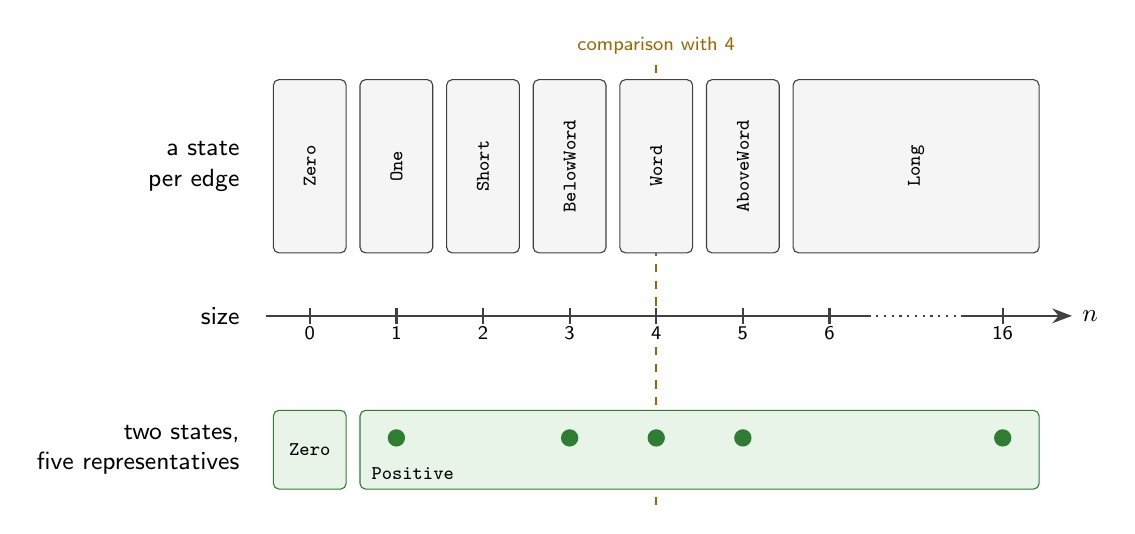
\begin{tikzpicture}[x=11mm, y=10mm, font=\small,
    old/.style={draw=flow, fill=groupfill, rounded corners=2pt},
    new/.style={draw=earsline, fill=earsfill, rounded corners=2pt},
    rep/.style={circle, fill=earsline, inner sep=0pt, minimum size=2.2mm},
    edge/.style={draw=codeline, dashed, thick},
    tick/.style={font=\scriptsize, fill=white, inner sep=1pt}]
  % The x coordinates of the sizes, not to scale.
  \def\xs{0/0, 1/1, 2/2, 3/3, 4/4, 5/5, 6/6, 8/16}
  % The comparison of the implementation.
  \draw[edge] (4, -1.2) -- (4, 4.4);
  \node[font=\scriptsize, text=codeline, above] at (4, 4.4)
    {comparison with 4};
  % The states of the item before the merge.
  \foreach \a/\b/\n in {0/0/Zero, 1/1/One, 2/2/Short, 3/3/BelowWord,
      4/4/Word, 5/5/AboveWord, 6/8/Long} {
    \draw[old] (\a-0.42, 2.0) rectangle (\b+0.42, 4.2);
    \node[rotate=90, font=\scriptsize\ttfamily] at ({(\a+\b)/2}, 3.1) {\n};
  }
  \node[anchor=east, align=right] at (-0.7, 3.1) {a state\\per edge};
  % The size axis.
  \draw[-{Stealth[length=2.5mm]}, thick, draw=flow] (-0.5, 1.2) -- (8.8, 1.2)
    node[right] {$n$};
  \foreach \x/\l in \xs {
    \draw[thick, draw=flow] (\x, 1.1) -- (\x, 1.3);
    \node[tick, below] at (\x, 1.1) {\l};
  }
  \fill[white] (6.45, 1.05) rectangle (7.55, 1.35);
  \draw[dotted, thick, draw=flow] (6.45, 1.2) -- (7.55, 1.2);
  \node[anchor=east] at (-0.7, 1.2) {size};
  % The classes and the representatives after the merge.
  \draw[new] (-0.42, -1.0) rectangle (0.42, 0.0);
  \node[font=\scriptsize\ttfamily] at (0, -0.5) {Zero};
  \draw[new] (0.58, -1.0) rectangle (8.42, 0.0);
  \node[font=\scriptsize\ttfamily, anchor=south west] at (0.6, -1.0)
    {Positive};
  \foreach \x in {1, 3, 4, 5, 8} {
    \node[rep] at (\x, -0.35) {};
  }
  \node[anchor=east, align=right] at (-0.7, -0.5)
    {two states,\\five representatives};
\end{tikzpicture}
\end{document}
